% Drawing 74/05-16 -- folder 74, batch 05, archive page 90 (PDF page 91).
% Transcription: Diagramme en forme de cube, flèches marquées $2$ ou $3$. En haut : $\mathrm{Car}_{d*}\simeq$ pav à \uncertain{trig pt}, recevant des flèches $2$ de $\mathrm{car}$ et de $\mathrm{Car}_{s*}\simeq$ pav.\ \uncertain{car} $\simeq$ pav $+$ trig ép ($\mathfrak{S}_3$). Au milieu : $\mathrm{hex}_{\Omega}\simeq$ tria $\Omega$ $\xleftarrow{3}\mathrm{hex}_{r'}\simeq\mathrm{car}_{r'}\simeq$ tria ép ($\mathfrak{S}_3$) ; $\mathrm{Car}\simeq$ pav pt. Puis $\mathrm{hex}$ ($\simeq$ tria) $\leftarrow\mathrm{hex}_{\mathrm{tr}*}$ ($\mathfrak{S}_3$) $\leftarrow\mathrm{hex}_{\mathrm{tr}\Omega}$ ($\simeq$ trig ép tria $\Omega$) $\xleftarrow{3}\mathrm{hex\,ép}$ ($\simeq$ trig ép tria ép, $\simeq$ pav ép ; $\mathfrak{S}_2$) ; $\mathrm{hex}_{d}$ ($\simeq\mathrm{Car}_{d}\simeq$ tria pt) $\leftarrow\mathrm{hex}_{s*}\leftarrow\mathrm{hex\,ép}$. En bas : $\mathrm{Pav\,coor}\simeq$ trig tria $\xleftarrow{3}\mathrm{hex}_{\mathrm{tr}}$ ($\mathfrak{S}_3$ ; $\simeq$ trig ép tria) $\xleftarrow{3}\mathrm{hex}_{s}$ ($\simeq$ tria ép ; $\mathfrak{S}_3$), trig tria pt $\simeq$ tria ; $\mathrm{Pav\,coor}\xrightarrow{2}\mathrm{Pav}$ ; trig $\Omega$ tria $\xleftarrow{3}$ tria $\Omega$. Les verticales $\mathrm{hex}\xrightarrow{3}\mathrm{Pav\,coor}$, $\mathrm{hex}_{\mathrm{tr}\Omega}\xrightarrow{2}\mathrm{hex}_{\mathrm{tr}}$, $\mathrm{hex}_{d}\xrightarrow{3}$ trig tria pt, $\mathrm{hex}_{s}\to$ tria $\Omega$ ; diagonales marquées $2$.
% Kind: cube-shaped arrow diagram. Method 2 (schematic redraw from the facsimile). Status: partial.
% Notes: Nodes placed where they stand, labels as the transcription reads them (uncertain words left as there), at \small; arrows with degrees 2 or 3 as seen. The bbox now holds the figure alone (the right half of the former bbox was blank paper), so the coordinates are those of the issue-73 redraw doubled. Still differs: the figure is in faint pencil and the directions of the diagonals are partly a reading. Nothing struck is drawn. Redrawn 2026-11-09 (issue 128): to check again.
% Coordinates: 1 unit = 1 mm = 1/100 of the crop width (bbox in page fractions: [0.15, 0.07, 0.55, 0.42]).
% Redrawn by Claude (claude-opus-5-5), issue #73, 2026-11-09; not checked by a human; not compiled (no TeX in the session).
% Rights: reproduces part of the work -- behind RENDER_TRANSCRIPTS, never published by itself.
\documentclass[tikz,border=3pt]{standalone}
\usepackage{amsmath,amssymb}
\usetikzlibrary{patterns,arrows.meta}
\tikzset{pencil/.style={black!45}, struck/.style={black!35}, mark/.style={circle,draw,inner sep=1.3pt}, pt/.style={circle,fill,inner sep=0.9pt}, opt/.style={circle,draw,fill=white,inner sep=1.1pt}}
\begin{document}
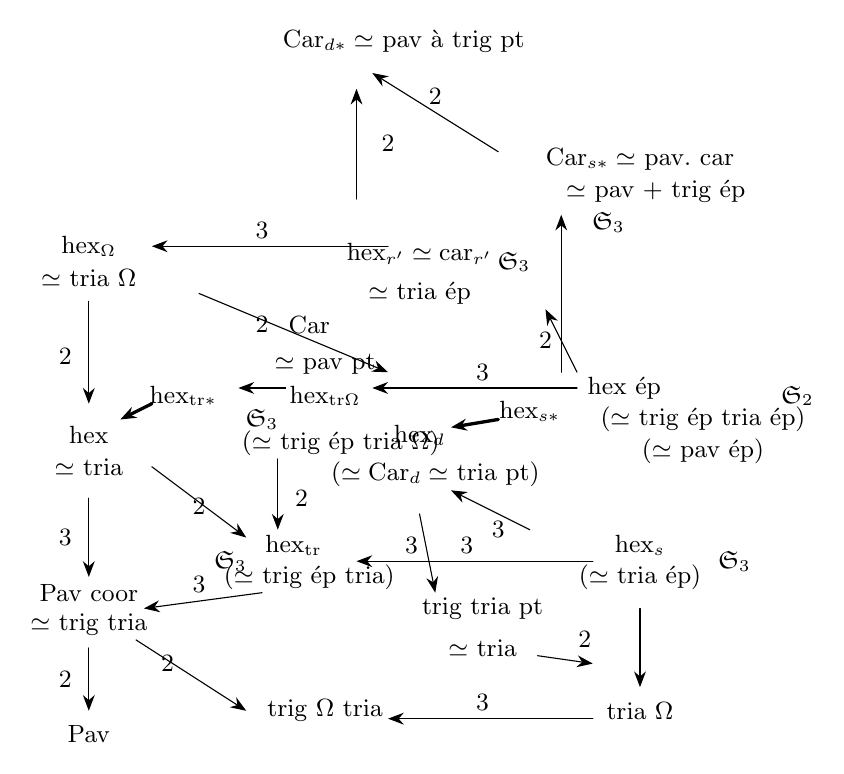
\begin{tikzpicture}[x=1mm,y=1mm,line cap=round,line join=round,font=\scriptsize]
\node[inner sep=1pt] at (56,-16) {\small $\mathrm{Car}_{d*}\simeq$ pav à trig pt};
\node[inner sep=1pt] at (44,-52) {\small Car};
\node[inner sep=1pt] at (46,-57) {\small $\simeq$ pav pt};
\node[inner sep=1pt] at (86,-31) {\small $\mathrm{Car}_{s*}\simeq$ pav.\ car};
\node[inner sep=1pt] at (88,-35) {\small $\simeq$ pav $+$ trig ép};
\node[inner sep=1pt] at (82,-39) {\small $\mathfrak S_3$};
\node[inner sep=1pt] at (58,-43) {\small $\mathrm{hex}_{r'}\simeq\mathrm{car}_{r'}$};
\node[inner sep=1pt] at (58,-48) {\small $\simeq$ tria ép};
\node[inner sep=1pt] at (70,-44) {\small $\mathfrak S_3$};
\node[inner sep=1pt] at (16,-42) {\small $\mathrm{hex}_\Omega$};
\node[inner sep=1pt] at (16,-46) {\small $\simeq$ tria $\Omega$};
\node[inner sep=1pt] at (16,-66) {\small hex};
\node[inner sep=1pt] at (16,-70) {\small $\simeq$ tria};
\node[inner sep=1pt] at (28,-61) {\small $\mathrm{hex}_{\mathrm{tr}*}$};
\node[inner sep=1pt] at (38,-64) {\small $\mathfrak S_3$};
\node[inner sep=1pt] at (46,-61) {\small $\mathrm{hex}_{\mathrm{tr}\Omega}$};
\node[inner sep=1pt] at (48,-67) {\small ($\simeq$ trig ép tria $\Omega$)};
\node[inner sep=1pt] at (84,-60) {\small hex ép};
\node[inner sep=1pt] at (94,-64) {\small ($\simeq$ trig ép tria ép)};
\node[inner sep=1pt] at (94,-68) {\small ($\simeq$ pav ép)};
\node[inner sep=1pt] at (106,-61) {\small $\mathfrak S_2$};
\node[inner sep=1pt] at (58,-66) {\small $\mathrm{hex}_d$};
\node[inner sep=1pt] at (60,-71) {\small ($\simeq\mathrm{Car}_d\simeq$ tria pt)};
\node[inner sep=1pt] at (72,-63) {\small $\mathrm{hex}_{s*}$};
\node[inner sep=1pt] at (16,-86) {\small Pav coor};
\node[inner sep=1pt] at (16,-90) {\small $\simeq$ trig tria};
\node[inner sep=1pt] at (16,-104) {\small Pav};
\node[inner sep=1pt] at (42,-80) {\small $\mathrm{hex}_{\mathrm{tr}}$};
\node[inner sep=1pt] at (44,-84) {\small ($\simeq$ trig ép tria)};
\node[inner sep=1pt] at (34,-82) {\small $\mathfrak S_3$};
\node[inner sep=1pt] at (86,-80) {\small $\mathrm{hex}_s$};
\node[inner sep=1pt] at (86,-84) {\small ($\simeq$ tria ép)};
\node[inner sep=1pt] at (98,-82) {\small $\mathfrak S_3$};
\node[inner sep=1pt] at (66,-88) {\small trig tria pt};
\node[inner sep=1pt] at (66,-93) {\small $\simeq$ tria};
\node[inner sep=1pt] at (46,-101) {\small trig $\Omega$ tria};
\node[inner sep=1pt] at (86,-101) {\small tria $\Omega$};
\draw[-{Stealth[length=2mm]}] (50,-36) -- (50,-22);
\node[inner sep=1pt] at (54,-29) {\small $2$};
\draw[-{Stealth[length=2mm]}] (68,-30) -- (52,-20);
\node[inner sep=1pt] at (60,-23) {\small $2$};
\draw[-{Stealth[length=2mm]}] (54,-42) -- (24,-42);
\node[inner sep=1pt] at (38,-40) {\small $3$};
\draw[-{Stealth[length=2mm]}] (41,-60) -- (35,-60);
\draw[-{Stealth[length=2mm]},very thick] (24,-62) -- (20,-64);
\draw[-{Stealth[length=2mm]}] (78,-60) -- (52,-60);
\node[inner sep=1pt] at (66,-58) {\small $3$};
\draw[-{Stealth[length=2mm]},very thick] (68,-64) -- (62,-65);
\draw[-{Stealth[length=2mm]}] (38,-86) -- (23,-88);
\node[inner sep=1pt] at (30,-85) {\small $3$};
\draw[-{Stealth[length=2mm]}] (80,-82) -- (50,-82);
\node[inner sep=1pt] at (64,-80) {\small $3$};
\draw[-{Stealth[length=2mm]}] (16,-93) -- (16,-101);
\node[inner sep=1pt] at (13,-97) {\small $2$};
\draw[-{Stealth[length=2mm]}] (80,-102) -- (54,-102);
\node[inner sep=1pt] at (66,-100) {\small $3$};
\draw[-{Stealth[length=2mm]}] (16,-74) -- (16,-84);
\node[inner sep=1pt] at (13,-79) {\small $3$};
\draw[-{Stealth[length=2mm]}] (40,-69) -- (40,-78);
\node[inner sep=1pt] at (43,-74) {\small $2$};
\draw[-{Stealth[length=2mm]}] (58,-76) -- (60,-86);
\node[inner sep=1pt] at (57,-80) {\small $3$};
\draw[-{Stealth[length=2mm]}] (86,-88) -- (86,-98);
\draw[-{Stealth[length=2mm]}] (16,-49) -- (16,-62);
\node[inner sep=1pt] at (13,-56) {\small $2$};
\draw[-{Stealth[length=2mm]}] (30,-48) -- (54,-58);
\node[inner sep=1pt] at (38,-52) {\small $2$};
\draw[-{Stealth[length=2mm]}] (24,-70) -- (36,-79);
\node[inner sep=1pt] at (30,-75) {\small $2$};
\draw[-{Stealth[length=2mm]}] (22,-92) -- (36,-101);
\node[inner sep=1pt] at (26,-95) {\small $2$};
\draw[{Stealth[length=2mm]}-] (80,-95) -- (73,-94);
\node[inner sep=1pt] at (79,-92) {\small $2$};
\draw[{Stealth[length=2mm]}-] (74,-50) -- (78,-58);
\node[inner sep=1pt] at (74,-54) {\small $2$};
\draw[-{Stealth[length=2mm]}] (72,-78) -- (62,-73);
\node[inner sep=1pt] at (68,-78) {\small $3$};
\draw[{Stealth[length=2mm]}-] (76,-38) -- (76,-58);
\end{tikzpicture}
\end{document}
